\documentclass[aspectratio=43]{beamer}

%\documentclass[handout]{beamer}
%% To make 4 per page
%\usepackage{pgfpages}
%\mode<handout>{\setbeamercolor{background canvas}{bg=white}}
%\pgfpagesuselayout{4 on 1}[letterpaper,landscape]%,border shrink=5mm]

\usetheme{default}
\usepackage{bm}
\usepackage{colortbl}

\usepackage{amsmath,amssymb,amsthm}
%\usepackage{subfigure}


% Fields and the like
\def\IC{\mathbb{C}}
\def\IF{\mathbb{F}}
\def\II{\mathbb{I}}
\def\IM{\mathbb{M}}
\def\IN{\mathbb{N}}
\def\IP{\mathbb{P}}
\def\IR{\mathbb{R}}
\def\IZ{\mathbb{Z}}

% Bold lowercase
\def\ba{\mathbf{a}}
\def\bb{\mathbf{b}}
\def\bc{\mathbf{c}}
\def\bd{\mathbf{d}}
\def\be{\mathbf{e}}
\def\bf{\mathbf{f}}
\def\bh{\mathbf{h}}
\def\bi{\mathbf{i}}
\def\bj{\mathbf{j}}
\def\bk{\mathbf{k}}
\def\bn{\mathbf{n}}
\def\bp{\mathbf{p}}
\def\br{\mathbf{r}}
\def\bs{\mathbf{s}}
\def\bu{\mathbf{u}}
\def\bv{\mathbf{v}}
\def\bw{\mathbf{w}}
\def\bx{\mathbf{x}}
\def\by{\mathbf{y}}
\def\bz{\mathbf{z}}

% Bold capitals
\def\bB{\mathbf{B}}
\def\bD{\mathbf{D}}
\def\bF{\mathbf{F}}
\def\bG{\mathbf{G}}
\def\bI{\mathbf{I}}
\def\bL{\mathbf{L}}
\def\bN{\mathbf{N}}
\def\bR{\mathbf{R}}
\def\bS{\mathbf{S}}
\def\bT{\mathbf{T}}
\def\bX{\mathbf{X}}

% Bold numbers
\def\b0{\mathbf{0}}

% Bold greek
\bmdefine{\bmu}{\bm{\mu}}
\def\bphi{\bm{\phi}}
\def\bvarphi{\bm{\varphi}}

% Bold red sentence
\def\boldred#1{{\color{red}\textbf{#1}}}
\def\defword#1{{\color{orange}\textbf{#1}}}

% Caligraphic letters
\def\A{\mathcal{A}}
\def\B{\mathcal{B}}
\def\C{\mathcal{C}}
\def\D{\mathcal{D}}
\def\E{\mathcal{E}}
\def\F{\mathcal{F}}
\def\G{\mathcal{G}}
\def\I{\mathcal{I}}
\def\L{\mathcal{L}}
\def\M{\mathcal{M}}
\def\P{\mathcal{P}}
\def\R{\mathcal{R}}
\def\S{\mathcal{S}}
\def\T{\mathcal{T}}
\def\U{\mathcal{U}}
\def\V{\mathcal{V}}

% tt font for code
\def\code#1{{\tt #1}}

% Operators and special symbols
\def\nbOne{{\mathchoice {\rm 1\mskip-4mu l} {\rm 1\mskip-4mu l}
{\rm 1\mskip-4.5mu l} {\rm 1\mskip-5mu l}}}
\def\cov{\ensuremath{\mathsf{cov}}}
\def\Var{\ensuremath{\mathsf{Var}\ }}
\def\Im{\textrm{Im}\;}
\def\Re{\textrm{Re}\;}
\def\det{\ensuremath{\mathsf{det}}}
\def\diag{\ensuremath{\mathsf{diag}}}
\def\nullspace{\ensuremath{\mathsf{null}}}
\def\nullity{\ensuremath{\mathsf{nullity}}}
\def\rank{\ensuremath{\mathsf{rank}}}
\def\range{\ensuremath{\mathsf{range}}}
\def\sgn{\ensuremath{\mathsf{sgn}}}
\def\Span{\ensuremath{\mathsf{span}}}
\def\tr{\ensuremath{\mathsf{tr}}}
\def\imply{$\Rightarrow$}
\def\restrictTo#1#2{\left.#1\right|_{#2}}
\newcommand{\parallelsum}{\mathbin{\!/\mkern-5mu/\!}}

% The beamer bullet (in base colour)
\def\bbullet{\leavevmode\usebeamertemplate{itemize item}\ }

% Theorems and the like
\newtheorem{proposition}[theorem]{Proposition}
\newtheorem{property}[theorem]{Property}
\newtheorem{importantproperty}[theorem]{Property}
\newtheorem{importanttheorem}[theorem]{Theorem}
%\newtheorem{lemma}[theorem]{Lemma}
%
%\usecolortheme{orchid}
\setbeamertemplate{theorems}[numbered]
%\usecolortheme{orchid}
%\setbeamertemplate{theorems}[ams style]
%\setbeamertemplate{theorems}[numbered]

%% Listings
\usepackage{listings}
\definecolor{mygreen}{rgb}{0,0.6,0}
\definecolor{mygray}{rgb}{0.5,0.5,0.5}
\definecolor{mymauve}{rgb}{0.58,0,0.82}
\definecolor{mygold}{rgb}{1,0.843,0}
\definecolor{myblue}{rgb}{0.537,0.812,0.941}

\definecolor{lgreen}{rgb}{0.6,0.9,.6}
\definecolor{lred}{rgb}{1,0.5,.5}

\lstloadlanguages{R}
\lstset{ %
  language=R,
  backgroundcolor=\color{black!95},   % choose the background color
  basicstyle=\footnotesize\ttfamily,        % size of fonts used for the code
  breaklines=true,                 % automatic line breaking only at whitespace
  captionpos=b,                    % sets the caption-position to bottom
  commentstyle=\color{mygreen},    % comment style
  escapeinside={\%*}{*)},          % if you want to add LaTeX within your code
  keywordstyle=\color{myblue},       % keyword style
  stringstyle=\color{mygold},     % string literal style
  keepspaces=true,
  columns=fullflexible,
  tabsize=4,
}
% Could also do (in lstset)
% basicstyle==\fontfamily{pcr}\footnotesize


% Get rid of navigation stuff
\setbeamertemplate{navigation symbols}{}

% Set footline/header line
\setbeamertemplate{footline}
{%
\quad p. \insertpagenumber \quad--\quad \insertsection\vskip2pt
}
% \setbeamertemplate{headline}
% {%
% \quad\insertsection\hfill p. \insertpagenumber\quad\mbox{}\vskip2pt
% }


\makeatletter
\newlength\beamerleftmargin
\setlength\beamerleftmargin{\Gm@lmargin}
\makeatother

%%%%%%% 
%% Definitions in yellow boxes
\usepackage{etoolbox}
\setbeamercolor{block title}{use=structure,fg=structure.fg,bg=structure.fg!05!bg}
\setbeamercolor{block body}{parent=normal text,use=block title,bg=block title.bg!20!bg}

\BeforeBeginEnvironment{definition}{%
	\setbeamercolor{block title}{fg=black,bg=yellow!20!white}
	\setbeamercolor{block body}{fg=black, bg=yellow!05!white}
}
\AfterEndEnvironment{definition}{
	\setbeamercolor{block title}{use=structure,fg=structure.fg,bg=structure.fg!20!bg}
	\setbeamercolor{block body}{parent=normal text,use=block title,bg=block title.bg!50!bg, fg=black}
}
\BeforeBeginEnvironment{importanttheorem}{%
	\setbeamercolor{block title}{fg=black,bg=red!20!white}
	\setbeamercolor{block body}{fg=black, bg=red!05!white}
}
\AfterEndEnvironment{importanttheorem}{
	\setbeamercolor{block title}{use=structure,fg=structure.fg,bg=structure.fg!20!bg}
	\setbeamercolor{block body}{parent=normal text,use=block title,bg=block title.bg!50!bg, fg=black}
}
\BeforeBeginEnvironment{theorem}{%
	\setbeamercolor{block title}{fg=white,bg=red!30!black}
	\setbeamercolor{block body}{fg=white, bg=red!10!black}
}
\AfterEndEnvironment{theorem}{
	\setbeamercolor{block title}{use=structure,fg=structure.fg,bg=structure.fg!20!bg}
	\setbeamercolor{block body}{parent=normal text,use=block title,bg=block title.bg!50!bg, fg=black}
}
\BeforeBeginEnvironment{importantproperty}{%
	\setbeamercolor{block title}{fg=black,bg=red!50!white}
	\setbeamercolor{block body}{fg=black, bg=red!30!white}
}
\AfterEndEnvironment{importantproperty}{
	\setbeamercolor{block title}{use=structure,fg=structure.fg,bg=structure.fg!20!bg}
	\setbeamercolor{block body}{parent=normal text,use=block title,bg=block title.bg!50!bg, fg=black}
}


%%%%%%%%%%%%%%%%%
\usepackage{tikz}
\usetikzlibrary{shapes,arrows}
\usetikzlibrary{positioning}
\usetikzlibrary{shapes.symbols,shapes.callouts,patterns}
\usetikzlibrary{calc,fit}
\usetikzlibrary{backgrounds}
\usetikzlibrary{decorations.pathmorphing,fit,petri}
\usetikzlibrary{automata}
\usetikzlibrary{fadings}
\usetikzlibrary{patterns,hobby}

\usepackage{pgfplots}
\pgfplotsset{compat=1.6}
\pgfplotsset{ticks=none}

\usetikzlibrary{decorations.markings}
\usetikzlibrary{arrows.meta}
\tikzset{>=stealth}

\tikzstyle{cloud} = [draw, 
ellipse,
fill=red!20, 
node distance=0.87cm,
minimum height=2em]
\tikzstyle{line} = [draw, 
-latex', 
color=yellow]


% Beginning of a section
% \AtBeginSection[]{
% 	{
% 		\setbeamercolor{background canvas}{bg=orange!10}
% 		\begin{frame}[noframenumbering,plain]
% 			\framesubtitle{\nameofthepart Chapter \insertromanpartnumber \ -- \iteminsert{\insertpart}}
% 			\tableofcontents[currentsection,currentsubsection]
% 		\end{frame}
% 	\addtocounter{page}{-1}
% 	%\addtocounter{framenumber}{-1} 
% 	}
% }


%%% SLIDES COLOURING

%\usecolortheme{owl}

\setbeamerfont{frametitle}{series=\bfseries}
\setbeamercolor{frametitle}{fg=black!05,bg=black}

\setbeamerfont{framesubtitle}{size=\normalfont\tiny}
\setbeamercolor{framesubtitle}{fg=black!05}

\setbeamercolor{background canvas}{bg=black}
\setbeamercolor{normal text}{fg=black!10}



\definecolor{bottomcolour}{rgb}{0.32,0.3,0.38}
\definecolor{middlecolour}{rgb}{0.08,0.08,0.16}
\definecolor{mycolor}{rgb}{0.4,0.4, 0.4}
% Beginning of a section
\AtBeginSection[]{
	{
		%\setbeamercolor{background canvas}[vertical shading][top=bottomcolour, middle=middlecolour, bottom=black]
		\setbeamertemplate{background canvas}[vertical shading][bottom=bottomcolour,top=black!20]
    % \setbeamertemplate{background canvas}{
    %   \begin{tikzpicture}%[remember picture,overlay]
    %     \shade[top color=yellow!75!green!33,
    %     bottom color=blue!66!green!33,
    %     middle color=blue!6!green!33]
    %   \end{tikzpicture}
    % }
    \begin{frame}[noframenumbering,plain]
			\framesubtitle{\nameofthepart Chapter \insertromanpartnumber \ -- \iteminsert{\insertpart}}
			\tableofcontents[currentsection,currentsubsection]
		\end{frame}
	\addtocounter{page}{-1}
	}
}
% Beginning of a section
\AtBeginSubsection[]{
	{
		%\setbeamercolor{background canvas}[vertical shading][top=bottomcolour, middle=middlecolour, bottom=black]
		%\setbeamertemplate{background canvas}[vertical shading][bottom=bottomcolour,top=black!20]
    \setbeamertemplate{background canvas}{
      \begin{tikzpicture}%[remember picture,overlay]
        \shade[top color=yellow!75!green!33,
        bottom color=blue!66!green!33,
        middle color=blue!6!green!33]
      \end{tikzpicture}
    }
    \begin{frame}[noframenumbering,plain]
			\framesubtitle{\nameofthepart Chapter \insertromanpartnumber \ -- \iteminsert{\insertpart}}
			\tableofcontents[currentsection,currentsubsection]
		\end{frame}
	\addtocounter{page}{-1}
	}
}

% Colours for special pages
\def\extraContent{yellow!20}

%% Allow to change slide colour
%% From: https://tex.stackexchange.com/questions/8043/change-the-background-color-of-a-frame-in-beamer
\defbeamertemplate*{background canvas}{mydefault}{%
  \ifbeamercolorempty[bg]{background canvas}{}{\color{bg}\vrule width\paperwidth height\paperheight}% copied beamer default here
}
\defbeamertemplate*{background canvas}{bg}{%
  \color{lightgray!20}\vrule width\paperwidth height\paperheight% added bg color
}
\BeforeBeginEnvironment{frame}{%
  \setbeamertemplate{background canvas}[mydefault]%
}
\makeatletter
\define@key{beamerframe}{bg}[true]{%
  \setbeamertemplate{background canvas}[bg]%
}
\makeatother
% Use with
%\begin{frame}
% \frametitle{Normal}
%\end{frame} 
%\begin{frame}[bg]
% \frametitle{With bg}
%\end{frame}


%% Vertical alignment on pages
%% From: https://tex.stackexchange.com/questions/148365/how-do-i-ask-beamer-to-exactly-fill-up-a-slide
%% Turn on with
%% \stretchon
%% (outside slide), and off with
%% \stretchoff
% \def\itemsymbol{$\blacktriangleright$}
% \let\svpar\par
% \let\svitemize\itemize
% \let\svenditemize\enditemize
% \let\svitem\item
% \let\svcenter\center
% \let\svendcenter\endcenter
% \let\svcolumn\column
% \let\svendcolumn\endcolumn
% \def\newitem{\renewcommand\item[1][\itemsymbol]{\vfill\svitem[##1]}}%
% \def\newpar{\def\par{\svpar\vfill}}%
% \newcommand\stretchon{%
%   \newpar%
%   \renewcommand\item[1][\itemsymbol]{\svitem[##1]\newitem}%
%   \renewenvironment{itemize}%
%     {\svitemize}{\svenditemize\newpar\par}%
%   \renewenvironment{center}%
%     {\svcenter\newpar}{\svendcenter\newpar}%
%   \renewenvironment{column}[2]%
%     {\svcolumn{##1}\setlength{\parskip}{\columnskip}##2}%
%     {\svendcolumn\vspace{\columnskip}}%
% }
% \newcommand\stretchoff{%
%   \let\par\svpar%
%   \let\item\svitem%
%   \let\itemize\svitemize%
%   \let\enditemize\svenditemize%
%   \let\center\svcenter%
%   \let\endcenter\svendcenter%
%   \let\column\svcolumn%
%   \let\endcolumn\svendcolumn%
% }
% \newlength\columnskip
% \columnskip 0pt



\title{Environmentally Transmitted Pathogens}
\subtitle{ODE models}
\author{Julien Arino}
\date{January 2023}


\begin{document}
%\stretchon

% The title page
\begin{frame}[noframenumbering,plain]
  \titlepage
\end{frame}
\addtocounter{page}{-1}

%%%%%%%%%%%%%%%%%%%%
%%%%%%%%%%%%%%%%%%%%
%%%%%%%%%%%%%%%%%%%%
%%%%%%%%%%%%%%%%%%%%
\section{The Kermack-McKendrick model}

\begin{frame}{Paper series worth reading}
Model here is a particular case in
\begin{itemize}
  \item Kermack \& McKendrick. \href{https://doi.org/10.1098/rspa.1927.0118}{A contribution to the mathematical theory of epidemics} (1927)
\end{itemize}
\vfill
That paper was followed by a series of ``Contributions to the mathematical theory of epidemics.''
\begin{itemize}
  \item \href{https://doi.org/10.1098/rspa.1932.0171}{II. The problem of endemicity} (1932)
  \item \href{https://doi.org/10.1098/rspa.1933.0106}{III. Further studies of the problem of endemicity} (1933)
  \item \href{https://doi.org/10.1017/S0022172400034902}{IV. Analysis of experimental epidemics of the virus disease mouse ectromelia} (1937)
  \item \href{https://doi.org/10.1017/S0022172400011918}{V. Analysis of experimental epidemics of mouse-typhoid; a bacterial disease conferring incomplete immunity} (1939)
\end{itemize}
\end{frame}

\begin{frame}{What is the \emph{size} of an epidemic?}
\bbullet 
If we are interested in the possibility that an epidemic occurs
\begin{itemize}
  \item Does an epidemic peak always take place?
  \item If it does take place, what is its size?
\end{itemize}
\vfill
\bbullet If an epidemic traverses a population, is everyone affected/infected?
\end{frame}


\begin{frame}{The SIR model without demography}
\bbullet The period of time under consideration is sufficiently short that demography can be neglected (we also say the model has \emph{no vital dynamics})
\vfill
\bbullet Differs from the SIS model, which includes demography (although it does consider it as being constant)
\vfill
\bbullet As in SIS model, individuals are either \emph{susceptible} to the disease or \emph{infected} (and \emph{infectious}) by the disease
\vfill
\bbullet However, after recovering or dying from the disease, individuals are \emph{removed} from the infectious compartment ($R$)
\vfill
\bbullet Incidence is of \defword{mass action} type, $\beta SI$
\end{frame}


\begin{frame}{The Kermack-McKendrick model}
This model is typically called the Kermack-McKendrick (KMK) SIR model 
\begin{subequations}\label{sys:KMK}
  \begin{align}
    S' &= -\beta SI \tag{1a}\label{sys:KMK_dS} \\
    I' &= \beta SI-\gamma I  \tag{1b}\label{sys:KMK_dI} \\
    R' &= \gamma I  \tag{1c}\label{sys:KMK_dR}
    \end{align}  
\end{subequations}
\vfill
\begin{center}
  \begin{tikzpicture}[scale=1.5, transform shape]
    \node [circle, fill=green!50, text=black] (S) {$S$};
    \node [circle, right=1.5cm of S, fill=red!90, text=black] (I) {$I$};
    \node [circle, right=1.5cm of I, fill=blue!90, text=black] (R) {$R$};
    %% Flows
    \path [line, very thick] (S) to node [midway, above] (TextNode) {$\beta SI$} (I);
    \path [line, very thick] (I) to node [midway, above] (TextNode) {$\gamma I$} (R);
  \end{tikzpicture}    
\end{center}
\end{frame}

%%%%%%%%%%%%%%%%%%%%
%%%%%%%%%%%%%%%%%%%%
%%%%%%%%%%%%%%%%%%%%
%%%%%%%%%%%%%%%%%%%%
\section{Mathematical analysis}

\begin{frame}{Reduction of the model}
  3 compartments, but when considered in detail, we notice that \emph{removed} do not have a direct influence on the dynamics of $S$ or $I$, in the sense that $R$ does not appear in \eqref{sys:KMK_dS} or \eqref{sys:KMK_dI}
  \vfill
  Furthermore, the total population (including deceased who are also in $R$) $N=S+I+R$ satisfies
  \[
  N'=(S+I+R)'=0
  \]
  Thus, $N$ is constant and the dynamics of $R$ can be deduced from $R=N-(S+I)$
  \vfill
  So we now consider
  \begin{subequations}\label{sys:KMK_2d}
    \begin{align}
      S' &= -\beta SI \label{sys:KMK_2d_dS}\\
      I' &= \beta SI-\gamma I  \label{sys:KMK_2d_dI}
      \end{align}
    \end{subequations}
\end{frame}

\begin{frame}{Equilibria}
  Let us consider the equilibria of
  \begin{subequations}
    \begin{align}
      S' &= -\beta SI 
      \tag{\ref{sys:KMK_2d_dS}} \\
      I' &= (\beta S-\gamma)I  
      \tag{\ref{sys:KMK_2d_dI}}
    \end{align}
  \end{subequations}
\vfill
  From \eqref{sys:KMK_2d_dI}
  \begin{itemize}
    \item either $\bar S=\gamma/\beta$ 
    \item or $\bar I=0$
  \end{itemize}
  \vfill
  Substitute into \eqref{sys:KMK_2d_dS}
  \begin{itemize}
    \item in the first case, $(\bar S,\bar I)=(\gamma/\beta,0)$ 
    \item in the second case, any $\bar S\geq 0$ is an EP
  \end{itemize}
  \vfill
  The second case is an \emph{issue}: the usual linearisation does not work when there is a \emph{continuum} of equilibria as the EP are not \emph{isolated}
\end{frame}


\begin{frame}{Another approach -- Study $dI/dS$}
  \begin{align}
  S' &= -\beta SI \tag{\ref{sys:KMK_2d_dS}}\\
  I' &= \beta SI-\gamma I  \tag{\ref{sys:KMK_2d_dI}}
  \end{align}
  \vfill
  What is the dynamics of $dI/dS$? 
  \begin{equation}
    \label{eq:KMK_dI_over_dS}
    \frac{dI}{dS}
    =\frac{dI}{dt}\frac{dt}{dS}
    =\frac{I'}{S'}
    =\frac{\beta SI-\gamma I}{-\beta SI}
    =\frac{\gamma}{\beta S}-1
  \end{equation}
 provided $S\neq 0$
  \vfill
  \textbf{Note --} Recall that $S$ and $I$ are $S(t)$ and $I(t)$.. \eqref{eq:KMK_dI_over_dS} thus describes the relation between $S$ and $I$ over solutions to the original ODE \eqref{sys:KMK_2d}
\end{frame}


\begin{frame}{}
  Integrate $\eqref{eq:KMK_dI_over_dS}$ and obtain trajectories in state space
  $$
  I(S)=\frac\gamma\beta \ln S-S+C
  $$
  with $C\in\mathbb{R}$
  \vfill
  IC $I(S_0)=I_0$ $\Rightarrow$ $C=S_0+I_0-\dfrac \gamma\beta \ln S_0$ and the solution to \eqref{sys:KMK} is, as a function of $S$
  \begin{align*}
  I(S)&=S_0+I_0-S+\frac\gamma\beta \ln \frac S{S_0} \\
  R(S)&=N-S-I(S)=R_0-\frac\gamma\beta \ln \frac S{S_0}
  \end{align*}
  (since $N_0=S_0+I_0+R_0$)
\end{frame}


\begin{frame}{}
  Trajectories of \eqref{sys:KMK_2d} in $(S,I)$-space, normalised, with IC $(S_0,1-S_0)$ and $\beta/\gamma=2.5$
  \vfill
\begin{center}
  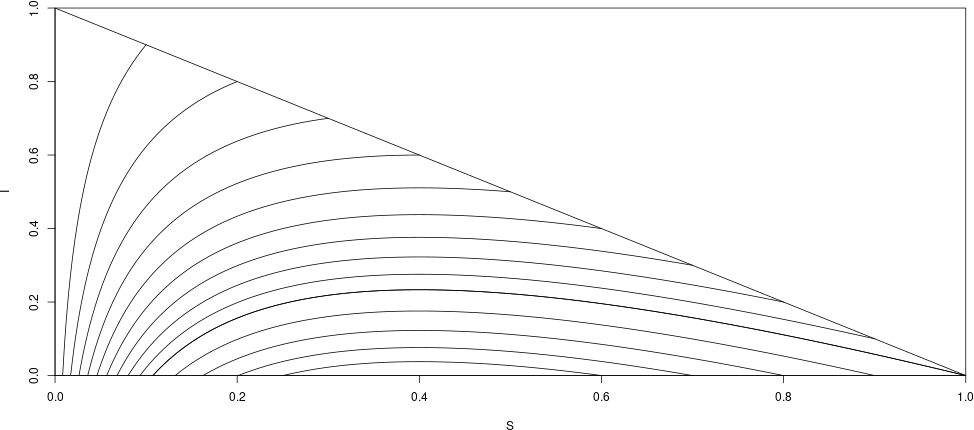
\includegraphics[width=\textwidth]{../FIGS/KMK_planar_trajectories.png}
\end{center}
\end{frame}


\begin{frame}{}
  Let us study
  $$
  I(S)=S_0+I_0-S+\frac\gamma\beta \ln \frac S{S_0} 
  $$
  We have
  $$
  \frac{d}{dS}I(S) = \frac{\gamma}{\beta S}-1
  $$
  So, in the previous curves, the max of $I(S)$ happens when $S=\gamma/\beta$ ($S=0.4$ in the example)
  \vfill
  At that point,
  $$
  I(S) = I_0+\left(
    1-\frac{1}{\R_0} - \frac{\ln(\R_0)}{\R_0}
  \right)S_0
  $$
\end{frame}


\begin{frame}{}
  \begin{theorem}[Epidemic or no epidemic?]
    Let $(S(t),I(t))$ be a solution to \eqref{sys:KMK_2d} and $\R_0$ defined by
    \begin{equation}\label{eq:R0_KMK}
    \R_0=\frac{\beta}{\gamma}S_0
    \end{equation}
    \vfill
    \begin{itemize}
      \item If $\R_0\leq 1$, then $I(t)\searrow 0$ when $t\to\infty$ 
      \item If $\R_0>1$, then $I(t)$ first reaches a maximum 
      \begin{equation}\label{eq:max_I}
        I_0+\left(
      1-\frac{1}{\R_0} - \frac{\ln(\R_0)}{\R_0}
      \right)S_0
      \end{equation}
      then goes to 0 as $t\to\infty$  
    \end{itemize}    
  \end{theorem}
\end{frame}

\begin{frame}[fragile]{}
\begin{lstlisting}
rhs_SIR_KMK <- function(t, x, p) {
  with(as.list(c(x, p)), {
    dS = - beta * S * I
    dI = beta * S * I - gamma * I
    dR = gamma * I
    return(list(c(dS, dI, dR)))
  })
}
# Condition initiale pour S (pour calculer R_0)
S0 = 1000
gamma = 1/14
# Set beta so that R_0 = 1.5
beta = 1.5 * gamma / S0 
params = list(gamma = gamma, beta = beta)
IC = c(S = S0, I = 1, R = 0)
times = seq(0, 365, 1)
sol <- ode(IC, times, rhs_SIR_KMK, params)  
\end{lstlisting}
\end{frame}


\begin{frame}[fragile]{}
\begin{lstlisting}
plot(sol[, "time"], sol[, "I"], type = "l",
main = TeX("Kermack-McKendrick SIR, $R_0=1.5$"),
xlab = "Time (days)", ylab = "Prevalence")
\end{lstlisting}
\begin{center}
  \includegraphics[width=\textwidth]{../FIGS/sol_SIR_KMK_R015}
\end{center}
\end{frame}


%%%%%%%%%%%%%%%%%%%%%%%%
%%%%%%%%%%%%%%%%%%%%%%%%
%%%%%%%%%%%%%%%%%%%%%%%%
%%%%%%%%%%%%%%%%%%%%%%%%
\section{Final size of an epidemic}

\begin{frame}{Final size of an epidemic}
  For a nonnegative valued integrable function $w(t)$, denote
  $$
  w_\infty = \lim_{t\to\infty}w(t),\qquad\hat w = \int_0^\infty w(t)\ dt
  $$
  Denote $w_0=w(0)$. In the subsystem
  \begin{align}
  S' &= -\beta SI \tag{\ref{sys:KMK_2d_dS}} \\
  I' &= \beta SI-\gamma I \tag{\ref{sys:KMK_2d_dI}} 
  \end{align}
  compute the sum of \eqref{sys:KMK_2d_dS} and \eqref{sys:KMK_2d_dI}, making sure to show time dependence $$
  \frac{d}{dt}(S(t)+I(t))=-\gamma I(t)
  $$
\end{frame}


\begin{frame}{}
  Integrate from 0 to $\infty$:
  $$
  \int_0^\infty\frac{d}{dt}(S(t)+I(t))\ dt=-\int_0^\infty\gamma I(t)dt 
  $$
  The left hand side gives
  $$
  \int_0^\infty\frac{d}{dt}(S(t)+I(t))\ dt
  = S_\infty+I_\infty-S_0-I_0 = S_\infty-S_0-I_0
  $$
  since $I_\infty=0$
  \vfill
  The right hand side takes the form
  $$
  -\int_0^\infty\gamma I(t)dt = -\gamma\int_0^\infty I(t)dt = -\gamma \hat I
  $$
  We thus have
  \begin{equation}
  \label{eq:KMK_final_size_step1}
  S_\infty-S_0-I_0 = -\gamma\hat I
  \end{equation}
\end{frame}



\begin{frame}{}
  Now consider \eqref{sys:KMK_2d_dS}:
  $$
  S' = -\beta SI
  $$
  Divide both sides by $S$:
  $$
  \frac{S'(t)}{S(t)} = -\beta I(t)
  $$
  Integrate from 0 to $\infty$:
  \begin{equation}
  \label{eq:KMK_final_size_step2}
  \ln S_\infty-\ln S_0 = -\beta \hat I
  \end{equation}
  Express \eqref{eq:KMK_final_size_step1} and \eqref{eq:KMK_final_size_step2} in terms of $-\hat I$ and equate
  $$
  \frac{\ln S_\infty-\ln S_0}{\beta}
  =
  \frac{S_\infty-S_0-I_0}{\gamma}
  $$
  Thus we have
  \begin{equation}
  \label{eq:final_size}
  (\ln S_0-\ln S_\infty)S_0 = (S_0-S_\infty)\R_0+I_0\R_0
  \end{equation}
\end{frame}



\begin{frame}{}
\begin{theorem}[Final size relation]
  Let $(S(t),I(t))$ be a solution to \eqref{sys:KMK_2d} and $\R_0$ defined by \eqref{eq:R0_KMK}
  \vskip0.5cm
  The number $S(t)$ of susceptible individuals is a nonincreasing function and its limit $S_\infty$ is the only solution in $(0,S_0)$ of the transcendental equation
  \begin{equation}\tag{\ref{eq:final_size}}
  (\ln S_0-\ln S_\infty)S_0 = (S_0-S_\infty)\R_0+I_0\R_0
  \end{equation}
\end{theorem}
\end{frame}



\begin{frame}{The (transcendantal) final size equation}
  Rewrite the final size equation
  \begin{equation}
    \tag{\ref{eq:final_size}}
  (\ln S_0-\ln S_\infty)S_0 = (S_0-S_\infty)\R_0+I_0\R_0
  \end{equation}
  as
  \begin{equation}
  \label{eq:final_size_2}
  T(S_\infty) =(\ln S_0-\ln S_\infty)S_0
  - (S_0-S_\infty)\R_0 -I_0\R_0
\end{equation}
\vfill
Thus, we seek the zeros of the function $T(S_\infty)$
\end{frame}



\begin{frame}{}
  We seek $S_\infty$ in $(0,S_0]$ s.t. $T(S_\infty)=0$, with
  \begin{equation}\tag{\ref{eq:final_size_2}}
    T(S_\infty) =(\ln S_0-\ln S_\infty)S_0
    - (S_0-S_\infty)\R_0 -I_0\R_0      
  \end{equation}
  \vfill
  Note to begin that 
  $$
  \lim_{S_\infty\to 0}T(S_\infty)=\lim_{S_\infty\to 0}-S_0\ln(S_\infty)=\infty
  $$
  \vfill
  Differentiating $T$ with respect to $S_\infty$, we get 
  $$
  T'(S_\infty)=\R_0-S_0/S_\infty
  $$ 
  \vfill
  When $S_\infty\to 0$, $\R_0-S_0/S_\infty<0$, so $T$ decreases to $S_\infty=S_0/\R_0$
  \vfill
  So if $\R_0\leq 1$, the function $T$ is decreasing on $(0,S_0)$, while it has a minimum if $\R_0>1$
\end{frame}



\begin{frame}{Case $\R_0\leq 1$}
  \begin{equation}\tag{\ref{eq:final_size_2}}
    T(S_\infty) =(\ln S_0-\ln S_\infty)S_0
    - (S_0-S_\infty)\R_0 -I_0\R_0      
  \end{equation}
  \vfill
  \bbullet We have seen that $T$ decreases on $(0,S_0]$
  \vfill
  \bbullet Also, $T(S_0)=-I_0\R_0<0$ ($I_0=0$ is trivial and not considered)
  \vfill
  \bbullet $T$ is continuous
  \vfill
  $\implies$ there exists a unique $S_\infty\in (0,S_0]$ s.t. $T(S_\infty)=0$
\end{frame}


\begin{frame}{Case $\R_0> 1$}
  \begin{equation}\tag{\ref{eq:final_size_2}}
    T(S_\infty) =(\ln S_0-\ln S_\infty)S_0
    - (S_0-S_\infty)\R_0 -I_0\R_0      
  \end{equation}
  \vfill
  \bbullet We have seen that $T$ decreases on $(0,S_0/\R_0]$
  \vfill
  \bbullet For $S_\infty\in[S_0/\R_0]$, $T'>0$
  \vfill
  \bbullet As before, $T(S_\infty)=-I_0\R_0$
  \vfill
  \bbullet $T$ is continuous
  \vfill
  $\implies$ there exists a unique $S_\infty\in (0,S_0]$ s.t. $T(S_\infty)=0$. More precisely, in this case, $S_\infty\in(0,S_0/\R_0)$
\end{frame}


\begin{frame}[fragile]{}
We solve numerically. We need a function
\begin{lstlisting}  
final_size_eq = function(S_inf, S0 = 999, I0 = 1, R_0 = 2.5) {
  OUT = S0*(log(S0)-log(S_inf)) - (S0+I0-S_inf)*R_0
  return(OUT)
}
\end{lstlisting}
and solve easily using \code{uniroot}, here with the values by default that we have set for the function
\begin{lstlisting}  
uniroot(f = final_size_eq, interval = c(0.05, 999))
$root
[1] 106.8819
$f.root
[1] -2.649285e-07
$iter
[1] 10
$init.it
[1] NA
$estim.prec
[1] 6.103516e-05
\end{lstlisting}
\end{frame}


\begin{frame}[fragile]{}
To use something else than the default values, e.g.,
\vfill
\begin{lstlisting}  
N0 = 1000
I0 = 1
S0 = N0-I0
R_0 = 2.4
uniroot(
  f = function(x) 
    final_size_eq(S_inf = x, 
                  S0 = S0, I0 = I0, 
                  R_0 = R_0),
  interval = c(0.05, S0))
\end{lstlisting}
\end{frame}


\begin{frame}[fragile]{A figure with all the information}
\begin{lstlisting}
S = seq(0.1, S0, by = 0.1)
fs = final_size(S, S0 = S0, I0 = I0, R_0 = R_0)
S_inf = uniroot(f = function(x) final_size_eq(S_inf = x, 
                                              S0 = S0, I0 = I0, 
                                              R_0 = R_0),
                interval = c(0.05, S0))
plot(S, fs, type = "l", ylab = "Value of equation (10)")
abline(h = 0)
points(x = S_inf$root, y = 0, pch = 19)
text(x = S_inf$root, y = 0, labels = "S_inf", adj = c(-0.25,-1))    
\end{lstlisting}
\end{frame}


\begin{frame}{$\R_0=0.8$}
\begin{center}
  \includegraphics[width=\textwidth]{../FIGS/KMK_final_size_R0_0p8}
\end{center}
\end{frame}


\begin{frame}{$\R_0=2.4$}
  \begin{center}
    \includegraphics[width=\textwidth]{../FIGS/KMK_final_size_R0_2p4}
  \end{center}
\end{frame}


\begin{frame}[fragile]{A little nicer}
\begin{lstlisting}
values = expand.grid(
  R_0 = seq(0.01, 3, by = 0.01),
  I0 = 1:100
)
values$S0 = N0-values$I0
L = split(values, 1:nrow(values))

values$S_inf = sapply(X = L, FUN = final_size)

values$taille_finale = values$S0-values$S_inf+values$I0
values$taux_attaque = (values$taille_finale / N0)*100

levelplot(taux_attaque ~ R_0*I0, data = values, 
          xlab="R_0", ylab = "I0",
          col.regions = viridis(100))  
\end{lstlisting}
(requires \code{lattice} and \code{viridis} librairies)
\end{frame}


\begin{frame}{Attack rate (in \%)}
  \begin{center}
    \includegraphics[width=\textwidth]{../FIGS/KMK_taux_attaque}
  \end{center}
\end{frame}


%%%%%%%%%%%%%%%%%%%%%%%%%%%
%%%%%%%%%%%%%%%%%%%%%%%%%%%
%%%%%%%%%%%%%%%%%%%%%%%%%%%
%%%%%%%%%%%%%%%%%%%%%%%%%%%
\section{Herd immunity}

\begin{frame}{The simplest vaccination model}
To implement vaccination in KMK, assume that vaccination reduces the number of susceptibles
\vfill
Let total population be $N$ with $S_0$ initially susceptible
\vfill
Vaccinate a fraction $p\in[0,1]$ of susceptible individuals
\vfill
Original IC (for simplicity, $R(0)=0$)
\begin{equation}\label{eq:IC_KMK_novacc}
IC: (S(0),I(0),R(0)) = (S_0,I_0,0)
\end{equation}
Post-vaccination IC 
\begin{equation}\label{eq:IC_KMK_vacc}
IC: (S(0),I(0),R(0)) = ((1-p)S_0,I_0,pS_0)
\end{equation}
\end{frame}


\begin{frame}{Vaccination reproduction number}
  Without vaccination
  \begin{equation}\tag{\ref{eq:R0_KMK}}
    \R_0=\frac{\beta}{\gamma}S_0
  \end{equation}
  \vfill
  With vaccination, denoting $\R_0^{\text{v}}$ the reproduction number,
  \begin{equation}
    \R_0^{\text{v}} = \frac{\beta}{\gamma}(1-p)S_0
  \end{equation}
  \vfill
  Since $p\in[0,1]$, $\R_0^{\text{v}}\leq\R_0$
\end{frame}


\begin{frame}{Herd immunity}
  Therefore
  \begin{itemize}
    \item $\R_0^{\textrm{v}}<\R_0$ if $p>0$ 
    \item To control the disease, $\R_0^{\text{v}}$ must take a value less than 1
  \end{itemize}
  \vfill
To make $\R_0^{\text{v}}$ less than 1
  \begin{equation}\label{eq:herd_immunity}
    \R_0^{\text{v}}<1 \iff p> 1-\frac{1}{\R_0}
  \end{equation}
  \vfill
  By vaccinating a fraction $p>1-1/\R_0$ of the susceptible population, we thus are in a situation where an epidemic peak is precluded (or, at the very least, the final size is reduced)
  \vfill
  This is \defword{herd immunity}
\end{frame}


\begin{frame}{An SIR model with vaccination}
  Take SIR model and assume the following
  \vfill
- Vaccination takes susceptible individuals and moves them directly into the recovered compartment, without them ever becoming infected/infectious
\vfill
- Birth = death
\vfill
- A fraction $p$ is vaccinated at birth
\vfill
- $f(S,I,N)=\beta SI$

%![width:600px center](https://raw.githubusercontent.com/julien-arino/omni-course-part1/main/FIGS/SIR_simple_vacc_blackBG.png)
\end{frame}


\begin{frame}{}
  %![bg left:30% width:350px](https://raw.githubusercontent.com/julien-arino/omni-course-part1/main/FIGS/SIR_simple_vacc_vertical_blackBG.png)

  \begin{subequations}\label{sys:SIR_demog_vacc}
    \begin{align}
      S' &= (1-p)dN-dS-\beta SI \label{sys:SIR_demog_vacc_dS}\\
      I' &= \beta SI -(d+\gamma)I \label{sys:SIR_demog_vacc_dI}\\
      R' &= pdN+\gamma I-dR \label{sys:SIR_demog_vacc_dR}
      \end{align}        
  \end{subequations}
\end{frame}

\begin{frame}{Computation of $\R_0$}
  - DFE, SIR: 
  $$
  E_0:=(S,I,R)=(N,0,0)
  $$
  - DFE, SIR with vaccination
  $$
  E_0^v:=(S,I,R)=
  \left((1-p)N,0,pN\right)
  $$
  
  Thus,
  - In SIR case
  $$
  \mathcal{R}_0=\frac{\beta N}{d+\gamma}
  $$
  - In SIR with vaccination case, denote $\R_0^{\text{v}}$ and
  $$
  \R_0^{\text{v}}=(1-p)\mathcal{R}_0
  $$    
\end{frame}



\begin{frame}{Herd immunity}
  Therefore 
  - $\R_0^{\textrm{v}}<\R_0$ if $p>0$
  - To control the disease, $\R_0^{\text{v}}$ must take a value less than 1, i.e.,
  \begin{equation}
    \R_0^{\text{v}}<1 \iff p> 1-\frac{1}{\R_0}
  \end{equation}
  \vfill
  By vaccinating a fraction $p>1-1/\R_0$ of newborns, we thus are in a situation where the disease is eventually eradicated
  \vfill
  This is \defword{herd immunity}
\end{frame}




%%%%%%%%%%%%%%%%%%%%%%%%%%%
%%%%%%%%%%%%%%%%%%%%%%%%%%%
%%%%%%%%%%%%%%%%%%%%%%%%%%%
%%%%%%%%%%%%%%%%%%%%%%%%%%%
\section{Last remarks}

\begin{frame}{To normalise or not to normalise?}
  \bbullet In the SIS of \href{}{Lecture 05} and here, since the total population is constant, it is possible to normalise to $N=1$
  \vfill
  \bbullet This can greatly simplify some computations
  \vfill
  \bbullet However, I am not a big fan: it is important to always have the ``sizes'' of objects in mind
  \vfill
  \bbullet If you do normalise, at least for a paper destined to mathematical biology, always do a ``return to biology'', i.e., interpret your results in a biological light, which often implies to return to original values
  \end{frame}

\begin{frame}{Where we are}
  \bbullet An \emph{endemic} SIS model in which the threshold $\R_0=1$ is such that, when $\R_0<1$, the disease goes extinct, whereas when $\R_0>1$, the disease becomes established in the population
  \vfill
  \bbullet An \emph{epidemic} SIR model (the KMK SIR) in which the presence or absence of an epidemic wave is characterised by the value of $\R_0$
  \vfill
  \bbullet The SIS and the KMK SIR have explicit solutions (in some sense). \textbf{This is an exception!}
\end{frame}


\end{document}